% This is LLNCS.DEM the demonstration file of
% the LaTeX macro package from Springer-Verlag
% for Lecture Notes in Computer Science,
% version 2.4 for LaTeX2e as of 16. April 2010
%
\documentclass{llncs}
%
\usepackage{makeidx}  % allows for indexgeneration
\usepackage{graphicx}
\usepackage{epstopdf}
%
\begin{document}




\maketitle              % typeset the title of the contribution

\begin{abstract}
Question Answering system has gradually become a new trend within the field of information retrieval and NLP. It outperforms the conventional search engines, for the system is able to answer users’ questions automatically and accurately. Question Answering system based on English corpus has developed rapidly, whereas the Chinese corpus based Question Answering system still has some problems remains to be solved. Thus, developing a new Question Answering model, which is characterized by dealing with features of Chinese corpus is extemely essentail. Different to the current deep learning model, our model uses the semantic and syntactic information in Chinese corpus and bases on the linearity of Chinese texts. Finally, our model turns out to perform better than other methods through experiments.\dots
\keywords{Question Answer, graph theory, Hamilton cycles}
\end{abstract}
%
\section{Introduction}
%


\section{Related Work}
% just test a cite~\cite{Severyn2015Learning}

\section{Methods}

%\subsection{Data Exploration}

\subsection{Data Exploration}

\subsubsection{Word Overlap and Character Overlap}
It is considered that the more keywords in questions are matched with those in the answer sentences, the more likely that the answer is the correct one.We have found that there are some relationships between the overlapped characters or words and the occurrence frequency of the correct answer after analysing the given corpus.

%\includegraphics[width=3in]{sensitive_simple_trec2013.pdf}

\begin{figure}[htb]
\centering
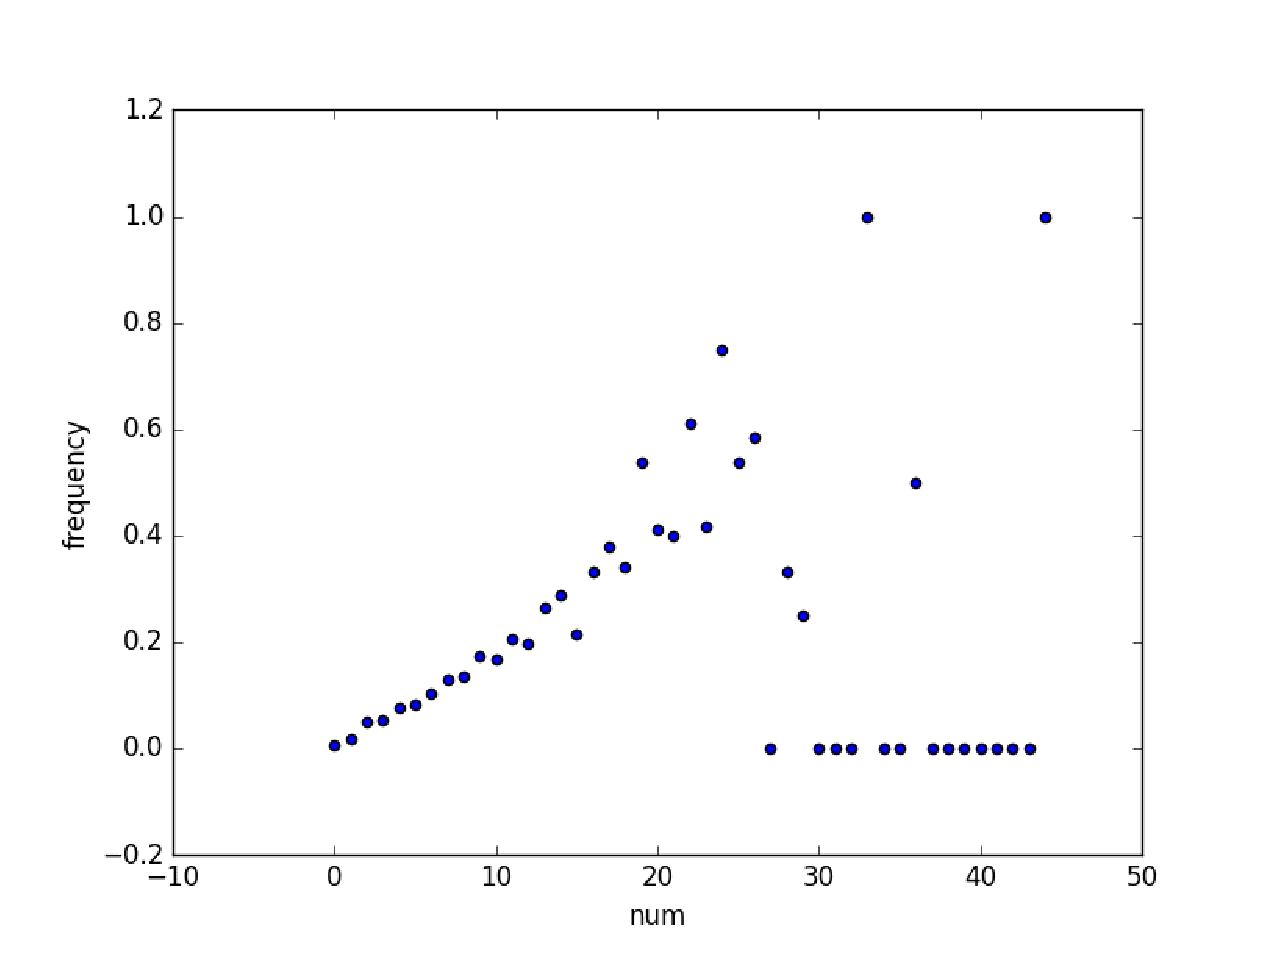
\includegraphics[width=4in]{figures/character_overlap.eps}
\caption{x-axis means the number of overlapped characters in both question and answer sentences.y-axis refers to the probable occurrence frequency of the target answer. Data are dispersed in the range between 22 and 50 because the samples are not enough.}
\label{fig:character_overlap}
\end{figure}


\begin{figure}
\centering
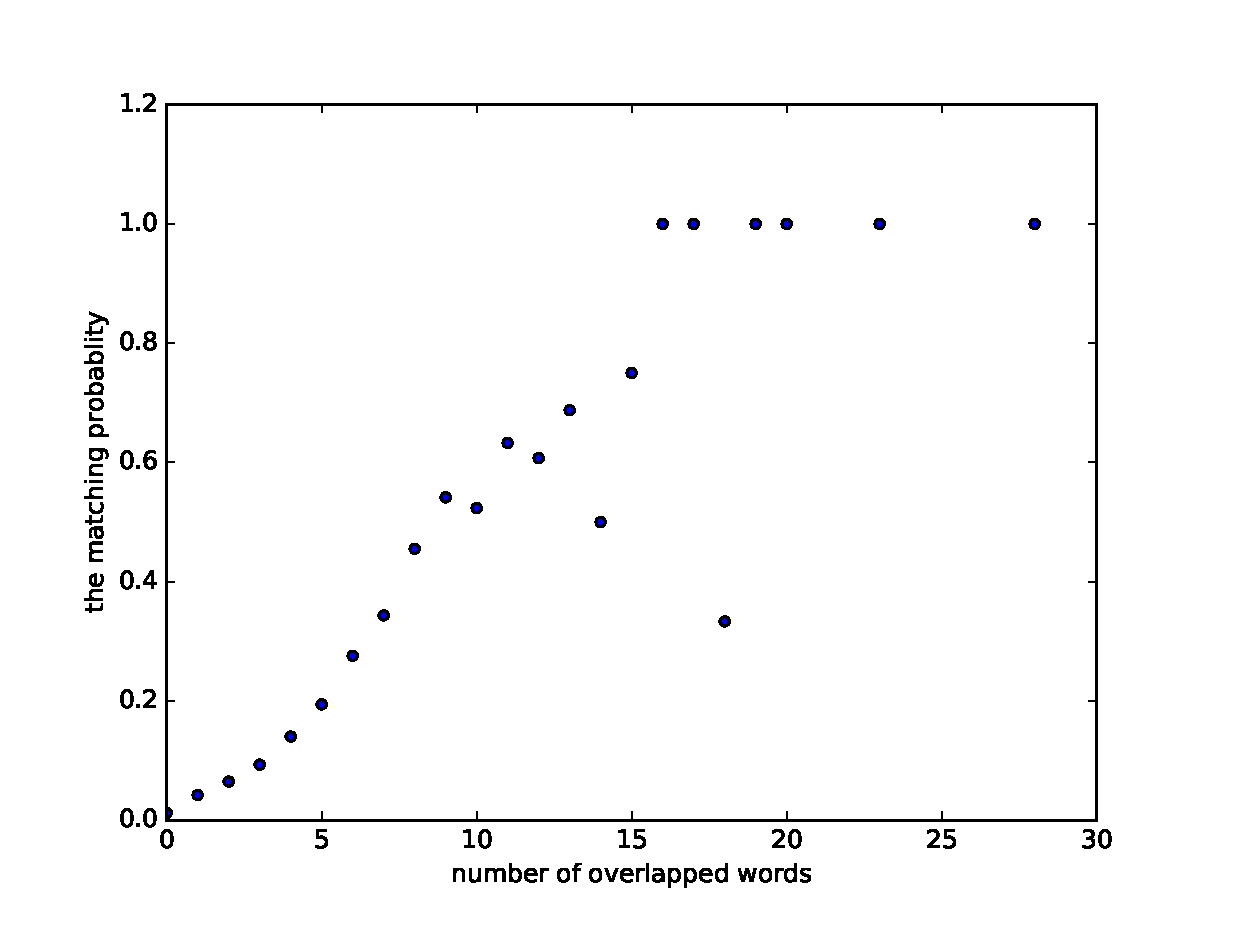
\includegraphics[width=4in]{figures/word_overlap.eps}
\caption{x-axis means the number of overlapped words in both question and answer sentences. y-axis refers to the probable occurrence frequency of the target answer. Data scatters after the number of 14 for the lack of words samples.}
\label{fig:word_overlap}
\end{figure}

We first segment the question and answer sentences into a series of characters and then count the total overlapped chatacers between the question and answer characters.As what have been shown in Fig. \ref{fig:character_overlap},it is concluded that there is a linear dependence between the correct answers’ frequency and overlapped characters.The same methods are also applied to the overlapped words and Fig. \ref{fig:word_overlap} illustrates that the more words are overlapped,the more likely that the answer is the correct one.

\subsubsection{Position Message in Overlapped Words}
In Chinese grammer, different grammatical elements are usually distributed in different position in a sentence.For example, in a classic question, the entities concerned usually turn up in the front of a sentence, which follows the interrogatives like ,”什么?几个?多少?”.People have various speaking habits when they organize a sentence in Chinese.For instance, premises are more inclined to appear first in one sentence.So it is reasonable to consider keywords’ position message when we are trying to get the degree of how question and answer matches. We try to give different weights to keywords in different positions in a sentence.Meanwhile, weights may also be concerned with words’ idf values, which means the discrimination of words.

\begin{figure}
\centering
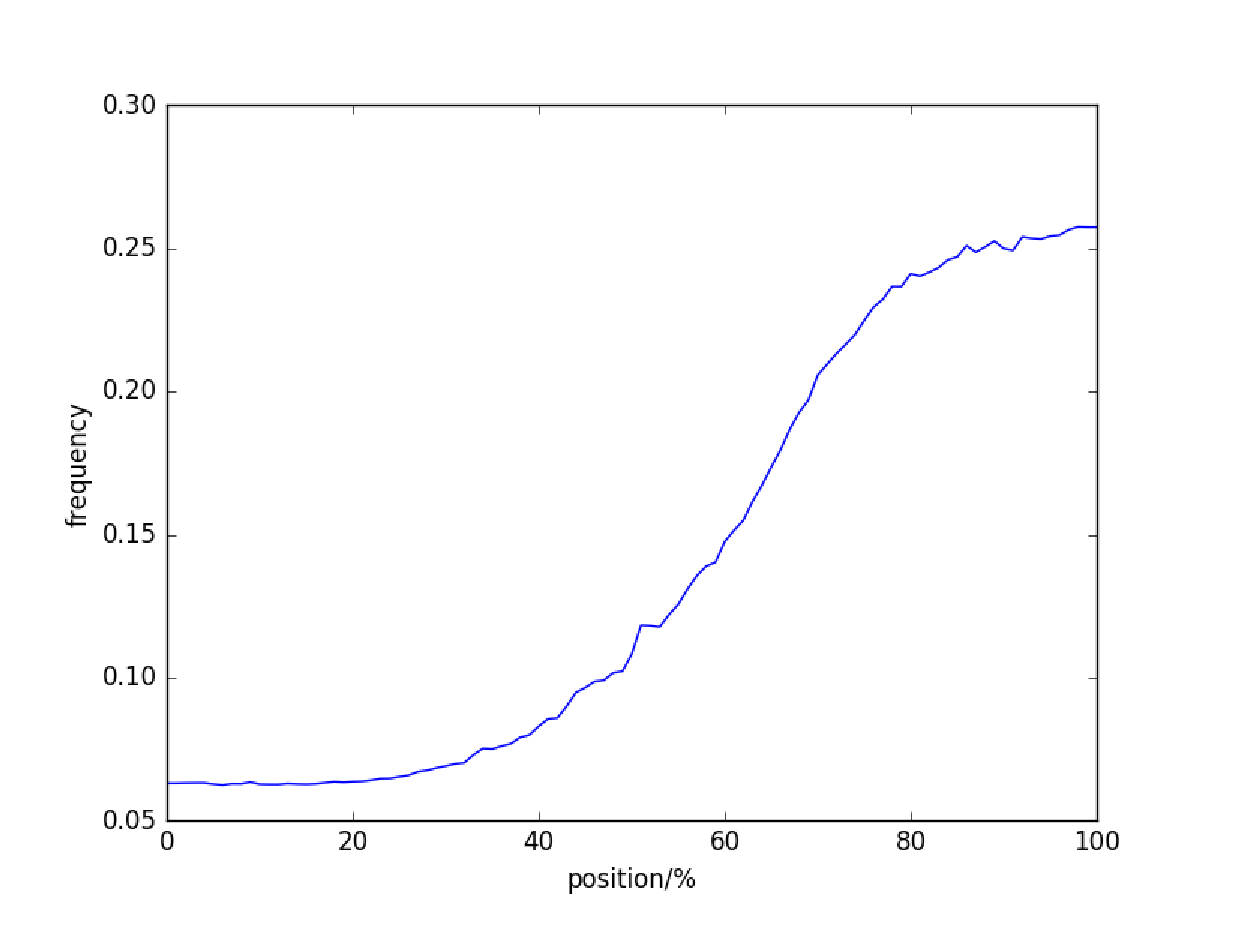
\includegraphics[width=4in]{figures/character_position.eps}
\caption{x-axis refers to the position of the overlapped characters in question sentences. x=0 means that the overlapped character is on the front of  a sentence.x=100\% means the overlapped character is on the back of a sentence.y-axis means the occurrence frenquency of correct answers.}
\label{fig:character_position}
\end{figure}

\begin{figure}
\centering
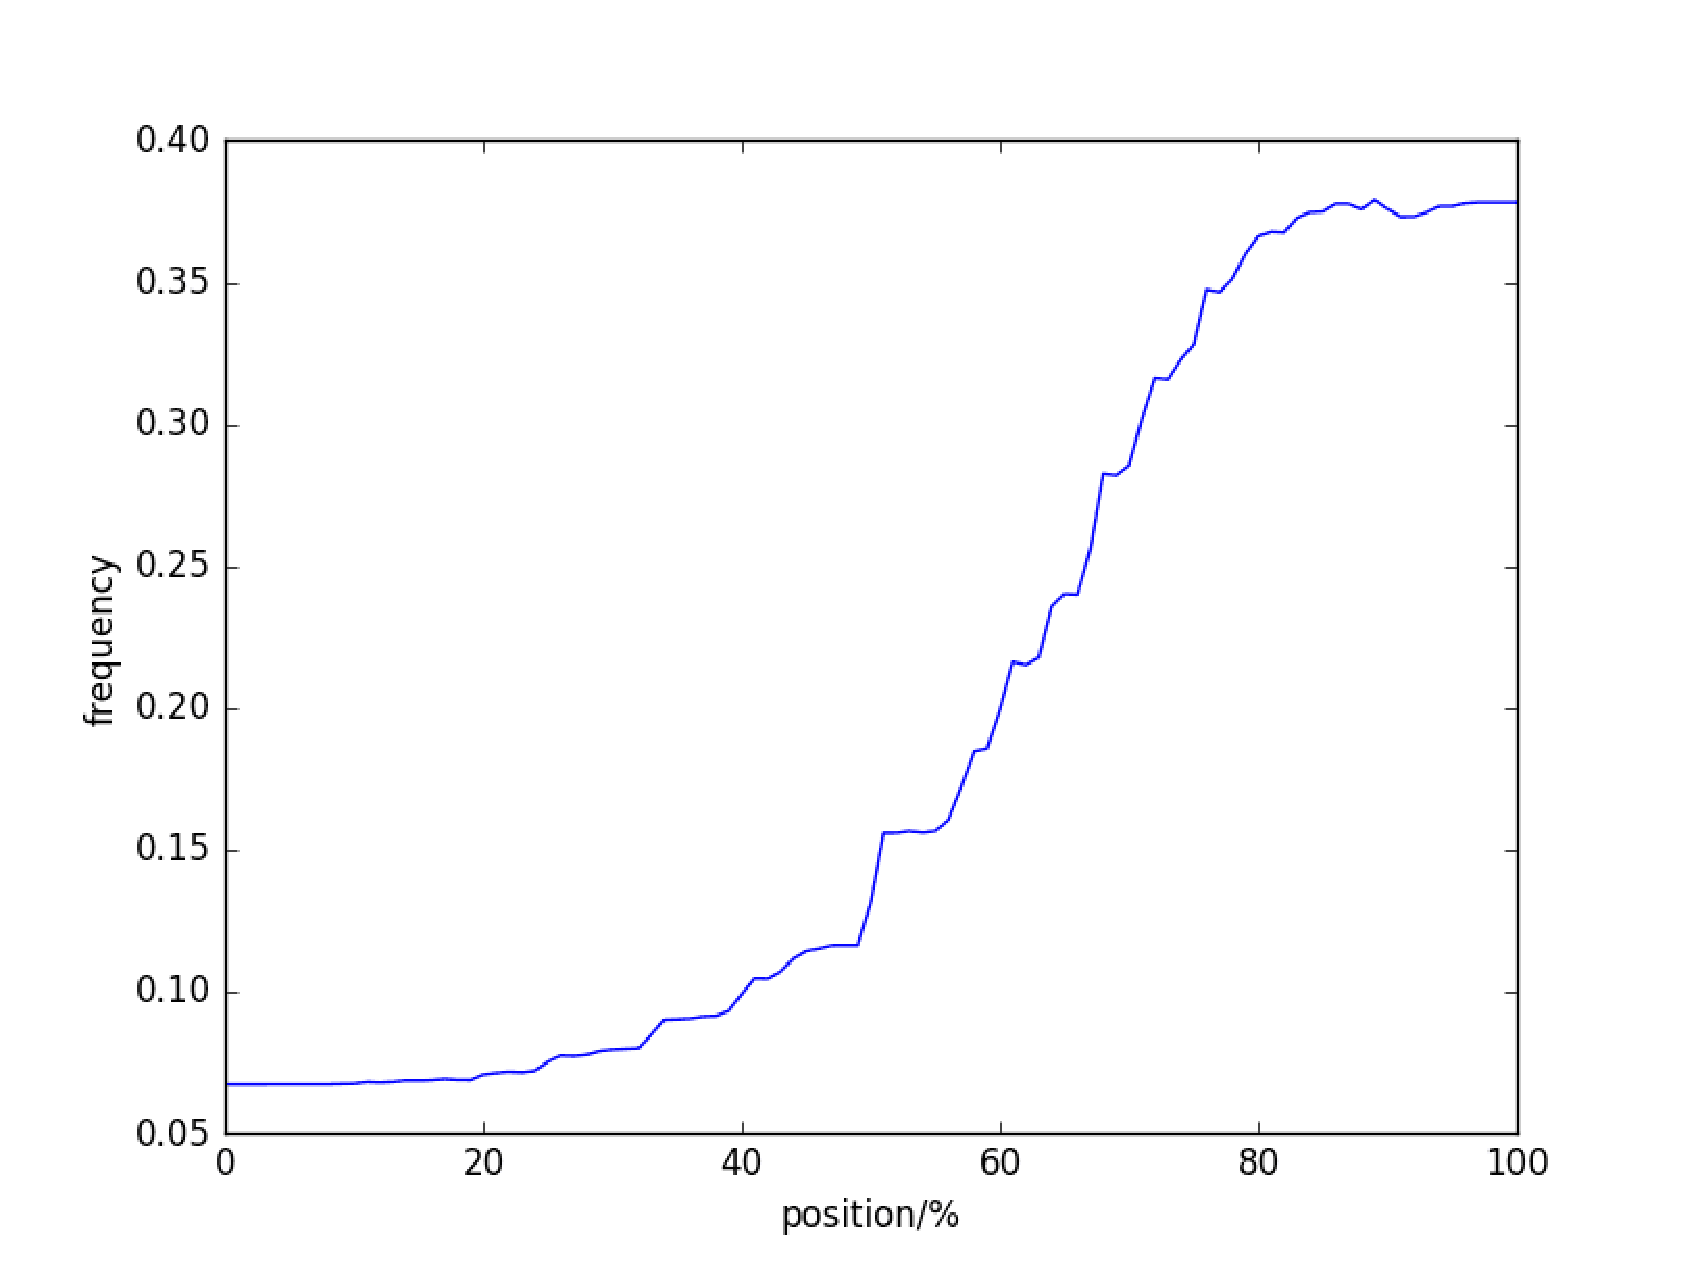
\includegraphics[width=4in]{figures/word_position.eps}
\caption{Similar to \ref{fig:character_position}, this figure shows the relationship between the position of the overlapped words in question sentences and the occurrence frenquency of correct answers.}
\label{fig:word_position}
\end{figure}



First we segment the question and answer sentences into characters (words) and then count the overlapped characters(words) and their position in both questions and answers.It is obvious that the overlapped characters(words) which often appear on the back of one sentence tends to be more important for us to find out the correct answer among answer text sets. We can also conclude from the two figures above that keywords or characters are more likely to appear on the back of the question sentences. Thus, we should give them higher weight than the rest.
Unforturnatly,word-overlap based method is still based on the hypothesis of word independence. Synonym rewriting based methods and translation model could model words which are extremely closed in meaning to some extent. To enumerate a rewriting templet(translate templet) of high quality and maturity is never a easy task. Current embedding methods, to some degree, model this kind of semantic similarity from semantic space of high dimensional, which will be analysed in section ??.
In Chinese,word group is composed of more Fined-grained characters. And word based overlap is a crude method to consider the correlation between words, which can be combined with other methods.


\subsection{Data Preprocessing}
We uses the pynlpir package(http://github.com/tsroten) to segment both the question sentences and the answer texts into word groups and we base our next work on these words.We then omit some of the stop words like “的,是,在…”in those word groups according to the stop words list(http://).It is necessary to cut out several meaningless words since it is of great help to extracting the words overlap feature.Finally, we get a processed dataset of words.


\subsection{Feature Extraction}
\subsubsection{Questions and Answers’ Type}
Question sentence’s type is usually a kind of vital signal.It is a prerequisite but not sufficient condition when distinguishing whether the given sentence is a correct answer or not. For example, for the question “中央大学的校长是谁?”,when the name entity related to person appears in one of the answer texts,it is probably that this sentence is the exact correct answer.But if little information is mentioned in the sentence,it is certain that the sentence will never be the target answer.Therefore, the type information is a prerequisite but not sufficient condition on defining the target answers. 
The answers to questions can be divided into 5 types(引用) and 3 of them are concerned with name entity, which are Person, Place, Organization.The others are Time and Number. In fact, a learning based way of finding out which type the question and answer belongs to could also make sense.However, we adopt the methods of extracting name entity to define the types of Person, Place and Organization and use model to find out the types of Time and Number because of the lack of supervised training and testing samples for learning. It turns out that our methods could cover more than 80\% cases and receive better results.
We adopt the LTP online API when naming entities.Meanwhile,we use templets to match keywords in anwers when naming entities in the types of Time and Number.
When we code,two methods are adopted.The first one is Dummp Number.The 5 types are viewed as 5 kinds of vectors. For each type, we use one-dimensional vector to indicate whether Question and Answer are matched or not.At the same time, or operation is made among the 5 types and the result is viewed as an one-dimensional vector for the reason that the result of each type is too sparse to count.
The second method is that the answer texts which are well matched by keywords in the question are marked as “1” and those which are not matched are marked as “0”.


\subsubsection{Overlap}
As QA pair match and Correlation have been mentioned in section??, namely,the more words are overlapped in both question and answer sentences,the more likely that the answer is the target one.
In these features, the removation of stop words seems to be vital due to the ignorance of the meaningless words.


\subsubsection{Other Conventional Methods}
Edit distance is usually used to measure the length of similar strings in English. While Jaccard index gives the similarity of two sets.And a sentence is often considered as a set of words.
The length of the answer texts is also a significant feature.


\subsubsection{Embedding}
We use embedding model as our main model.Embedding means to embed words into a high dimensional semantic space, which makes it easier to find the relationship between words. Sentence is simply considered to have been lapped by words linearly. As what have been mentioned in section??, we will give different weights to different words,which depends on their position, semantic structure and idf.


\subsection{Model Selection}
We have presented various fundamental features in last chapter,which will directly effect the degree of how question and answer matches.We adopt a linear regression model to integrate those features.While some integrated learning methods like Ada Boost and bagging models are also used. 



\section{Experimental results}




\section{Discussion and Conclution}








%
% ---- Bibliography ----
%
\begin{thebibliography}{}
%
\bibitem{Rodriguez.{2010}}
Open Source Cloud Computing Tools: A Case Study with a Weather Application
Rodriguez-Martinez, M.; Seguel, J.; Greer, M.
Cloud Computing (CLOUD), 2010 IEEE 3rd International Conference on
Year: 2010
% \bibliography{nlpcc_qa}
% \bibliographystyle{IEEEtran}

\end{thebibliography}



\end{document}
